\documentclass{jlreq}
\usepackage[dvipdfmx]{graphicx}
\usepackage[dvipdfmx]{color}
\usepackage[dvipdfmx]{hyperref}
\usepackage{amsmath}
\usepackage{geometry}
\usepackage{float}
\usepackage{array}
\usepackage{caption}
\usepackage{hyperref}
\usepackage{url}
\usepackage{listings}
\renewcommand{\lstlistingname}{リスト}
\linespread{1.2}
\numberwithin{equation}{section}
\counterwithin{figure}{section}
\counterwithin{table}{section}
\ModifyHeading{section}{before_space=20pt, after_space=20pt}
\ModifyHeading{subsubsection}{before_space=15pt, after_space=20pt}
\begin{document}

\section{目的}
ハードウェア記述言語VHDLを用いて、ストップウオッチの機能あるいは回路構成を記述し、それをFPGA上に実現することにより、ディジタル回路の動作原理ならびにその設計手順を理解する。また、設計・シミュレーション・実機検証の一連の工程を通じて、FPGA開発の実践的なスキルを習得し、効率的なデバッグ手法や設計の最適化についても学ぶ。

\section{原理}
\subsection{FPGAの原理}
FPGA(Field Programmable Gate Array)は、ユーザーが回路構成を自由に書き換えられる集積回路である。FPGA内部には多数のロジックブロック(論理素子)と、それらを相互接続する配線(インターコネクト)、そして設定情報を保持する構成メモリが組み込まれている。ユーザーはHDL(ハードウェア記述言語)を使って回路設計を行い、そのデータをFPGAに書き込むことで、加算器やカウンタ、プロセッサなど多様なデジタル回路を構成することができる。これにより、専用ICのようなハードウェアの高速性と、ソフトウェアの柔軟性を両立できる。(1)

FPGAのチップの内では、論理機能を実現することができ、EmbeddedArrayBlock(EAB)およびLogicArrayBlock(LAB)、ならびにそれらを接続するためのFastTrack列配線および行配線が、図2.1に示すように規則的に配置されている。

\begin{figure}[H]
  \centering
  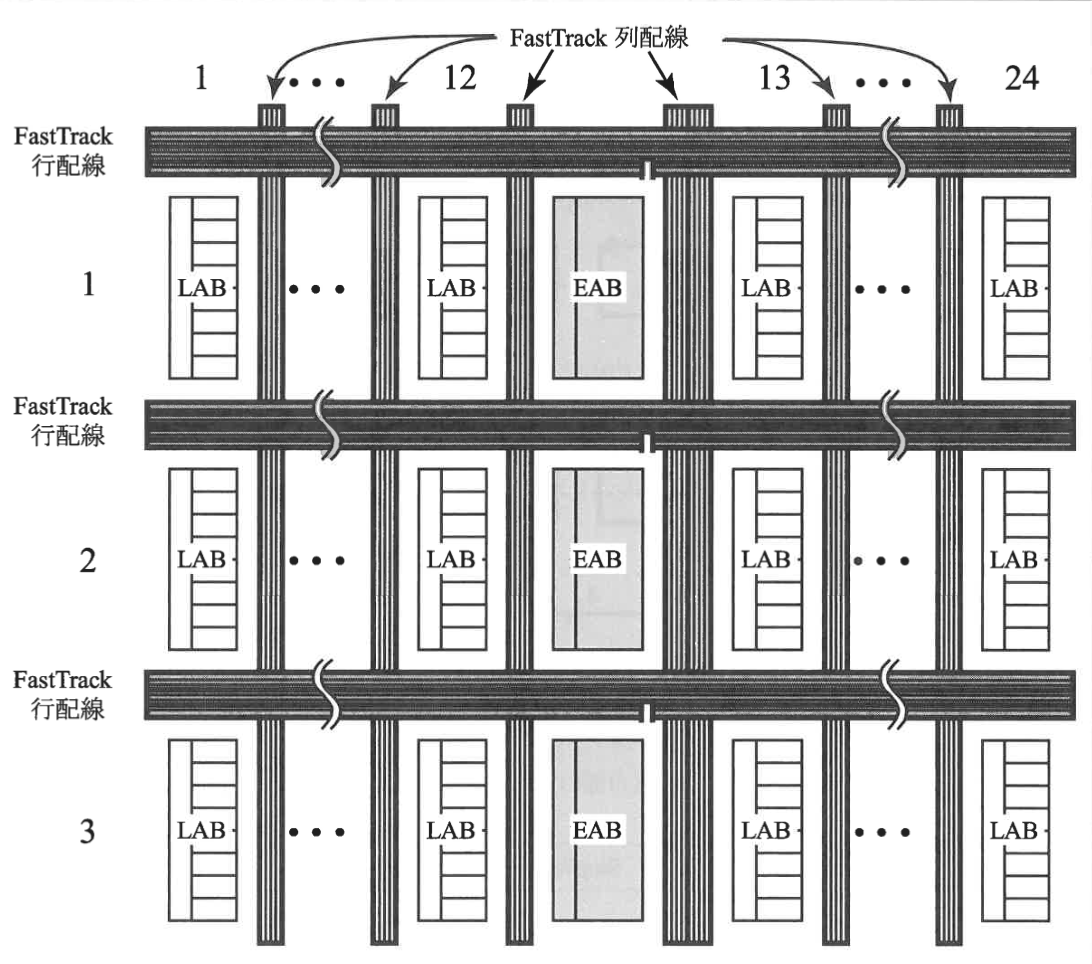
\includegraphics[width=0.7\textwidth]{assets/EP1K10_stracture.png}
  \caption{EP1K10の構造}
\end{figure}

EP1K10は3行25列構造で、各行にEABが1個、LABが24個配置されている。FastTrack配線は高速伝送が可能で、行配線は144本、列配線は通常24本だが、EAB横は48本となっている。EABは8入力16出力の任意関数を実現可能で、RAMやFIFOなどのメモリ機能やデータ処理にも利用できる。例えば、1つのEABで256x16ビットや512x8ビットのRAMを構成可能で、複数のEABを組み合わせることでより大容量のRAMも実現できる。

\subsection{実験で作成したStopWatchのモジュール構成と動作原理}
今回の実験で作成するStopWatchのモジュールは、FPGA ボード「DE10-Lite」を用いて構成されている。
ボードの主な構成要素としては、ストップウォッチの始動・停止用となるスイッチSW1(上側のボタンスイッチ)、押されたら計測時間および7セグメントLEDの表示を0に戻すリセット用のSW2(下側のボタンスイッチ)、時間の表示をする3つの7セグメントLEDがある。

また、今回作成するStopWatch回路の構造を図2.2に示す。

\begin{figure}[H]
  \centering
  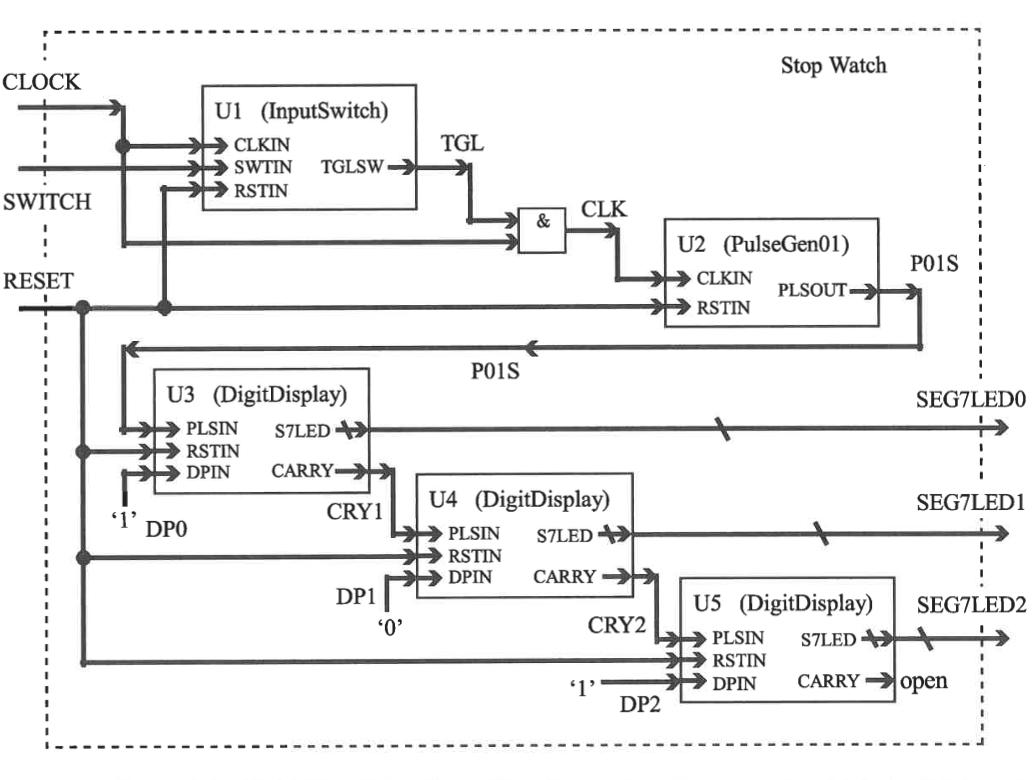
\includegraphics[width=0.9\textwidth]{assets/StopWatch_kairo.png}
  \caption{StopWatch回路の構造}
\end{figure}

ユニットU1では、クロック信号(今回実験で使用するボードでは50MHz)とスイッチ入力(SW1,SW2)を受け取り、値に応じてU2に情報を送っている。
U2ではクロック信号をもとに、適切なパルスを出力するようになっており、U3からU5ではパルス信号の入力を元に7セグメントLEDへの出力および小数点の表示、桁上げ処理などを行っている。

\section{実験結果}

\subsection{実験手順}

\subsubsection{VHDLコードの作成}
サブモジュールである周期0.1秒のパルス発生回路(PulseGen01)をVHDLで記述し、PulseGen01.vhd)として作成する。

\subsubsection{コンパイルとデバッグ}
Quartus Primeを用いてVHDLコードをコンパイルし、FPGAに実装可能な回路へ変換する。コンパイル時にエラーが発生した場合は、デバッグを行い記述を修正する。

\subsubsection{シミュレーションによる動作確認}
Quartus Primeのシミュレーション機能を利用して、設計した回路が仕様通り動作するか確認する。この際、実際の時間単位ではシミュレーションに時間がかかりすぎるのでパルス周期等を調整し、シミュレーションをしやすくする。

\subsubsection{FPGAへの書き込みとボード上での実機動作確認}
Quartus Primeから実機(ボード)に書き込み、実際のハードウェア上で動作を確認する。

\subsection{実験結果}
\subsubsection{使用した2種類のPulseGen01のプログラムリストと処理フローおよびその役割}
使用した2種類のPulseGen01のリストを図3.1,3.2に示す。

\begin{figure}[H]
  \centering
  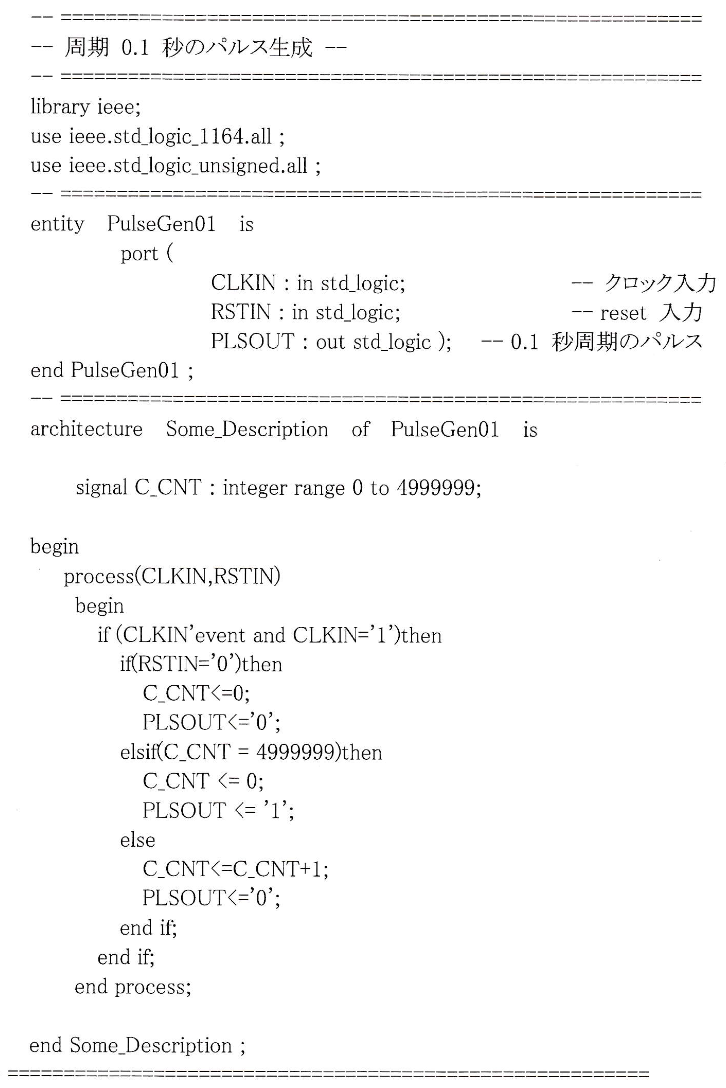
\includegraphics[width=0.8\textwidth]{assets/PulseGen01.png}
  \caption{PulseGen01のプログラムリスト(同期式)}
\end{figure}

\begin{figure}[H]
  \centering
  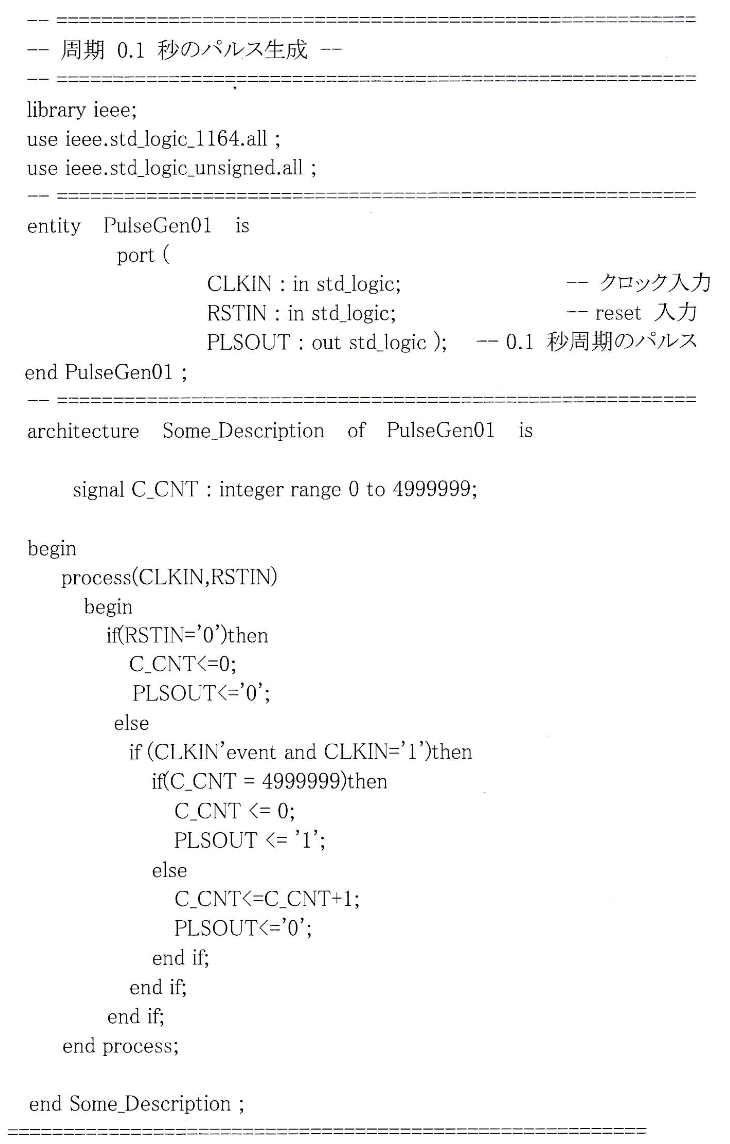
\includegraphics[width=0.8\textwidth]{assets/PulseGen02.png}
  \caption{PulseGen01のプログラムリスト(非同期式)}
\end{figure}

またこれらのプログラムの処理フローを図3.3,3.4に示す

\begin{figure}[H]
  \centering
  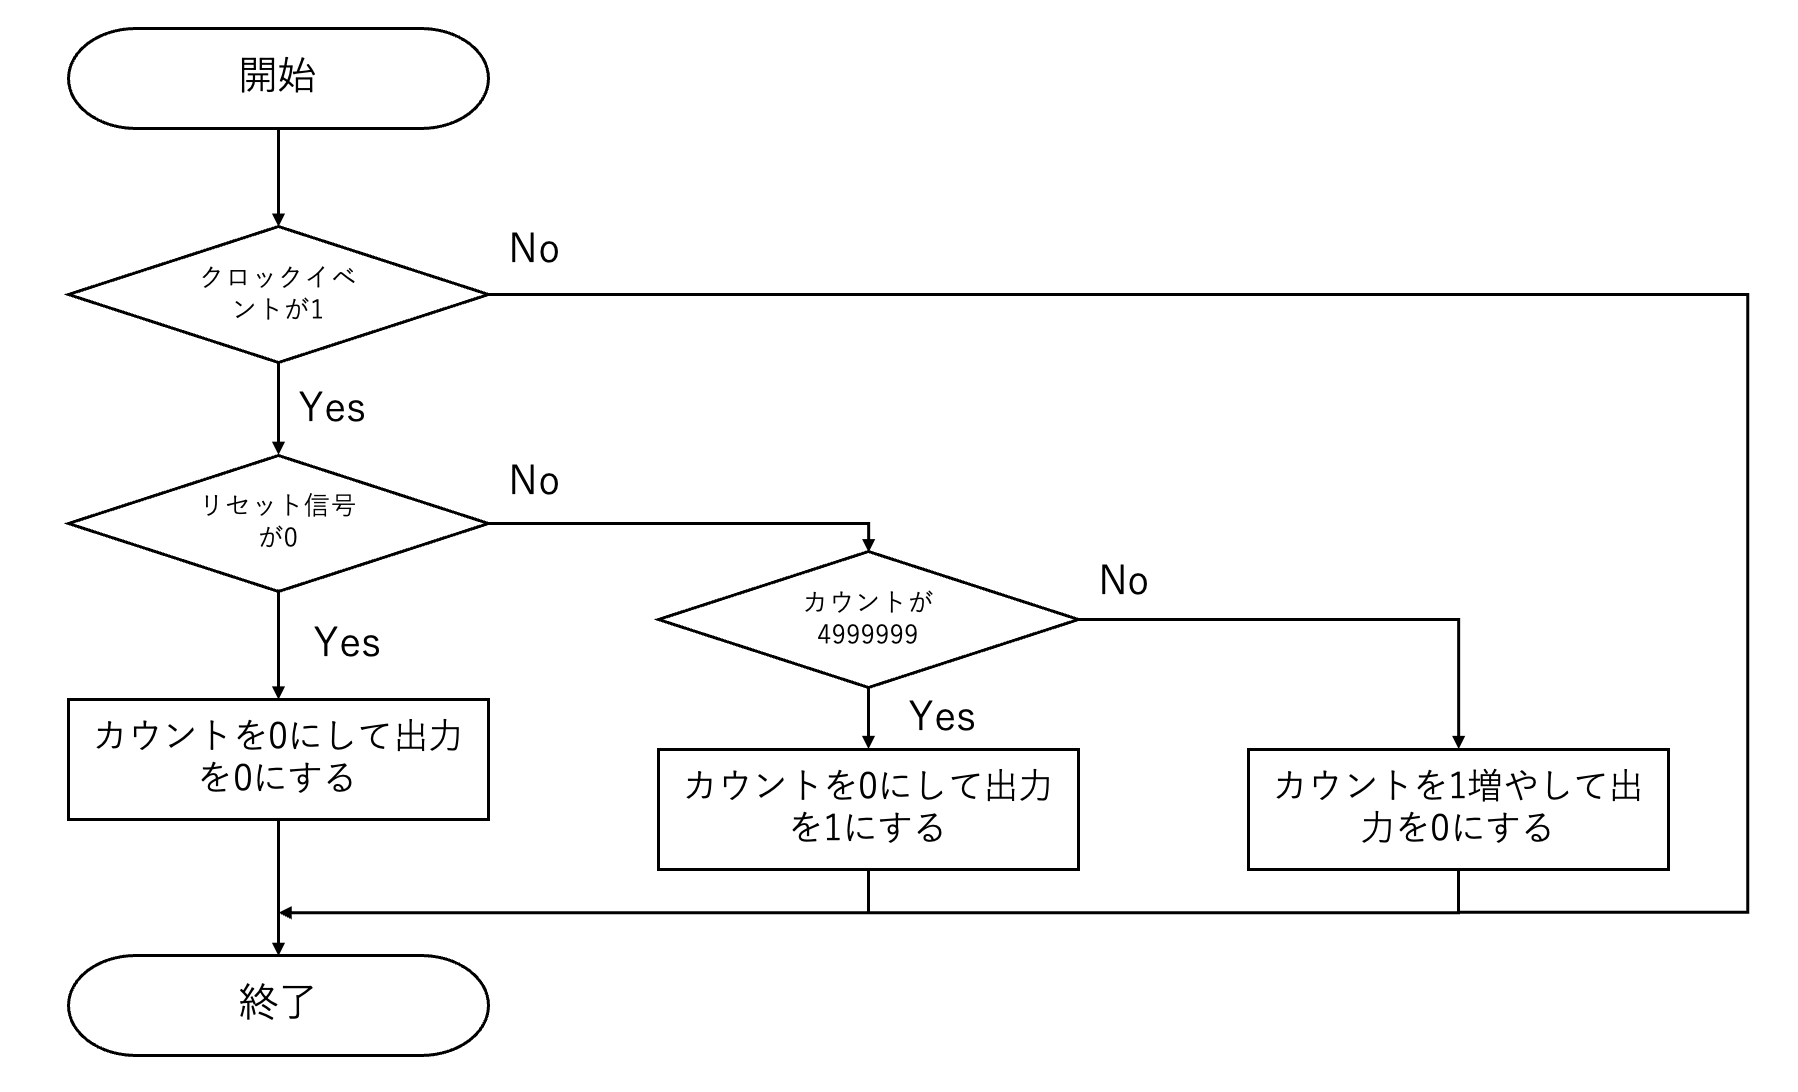
\includegraphics[width=\textwidth]{assets/flowchart01.png}
  \caption{PulseGen01の処理フロー(同期式)}
\end{figure}

\begin{figure}[H]
  \centering
  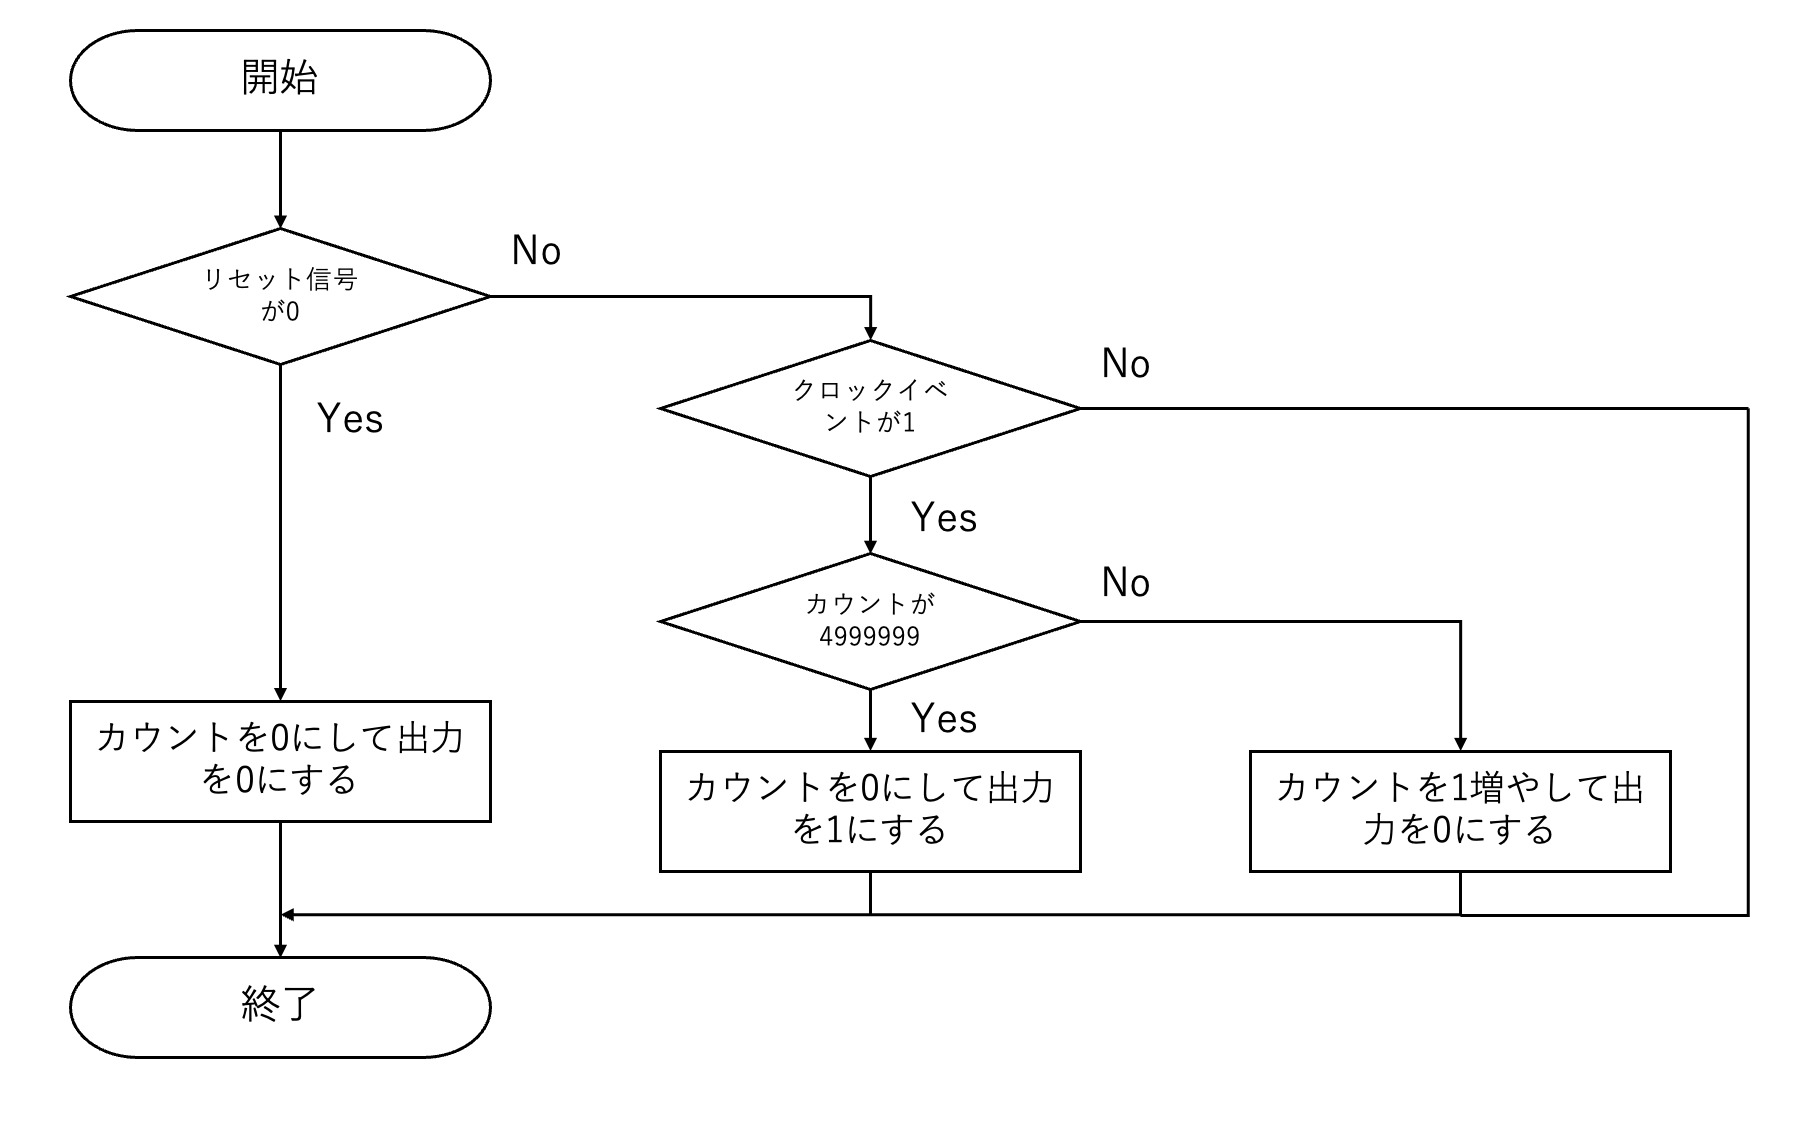
\includegraphics[width=\textwidth]{assets/flowchart02.png}
  \caption{PulseGen01の処理フロー(非同期式)}
\end{figure}

図3.3に示されているのは、PulseGen01の同期式処理フローである。このフローでは、すべての処理がクロックイベントに同期して実行される。すべての条件分岐や処理がクロックイベントによって制御されており、タイミングの一貫性が保たれているため、ハードウェア的に安定した動作が期待できる構成である。

一方、図3.4に示されているのは、PulseGen01の非同期式処理フローである。この処理フローでは、まずクロックとは無関係にリセット信号の状態が判定される。リセット信号がアクティブである場合、ただちにカウント値と出力は0に初期化される。リセット信号がアクティブでない場合にのみ、クロックイベントの有無が判定され、以降の処理は同期式と同様にカウント値に応じて動作する。非同期式の利点は、リセット処理がクロックに依存せず即座に反映される点にあるが、一方でタイミング制御が難しくなる可能性もあるため、安定性の観点では同期式に劣る場合がある。\\

表3.1に、同期式と非同期式のシミュレーション結果の比較を示す。

\begin{table}[H]
\centering
\caption{同期式と非同期式の解析結果の比較}
\begin{tabular}{|c|c|c|}
\hline
項目 & 同期式 & 非同期式 \\ \hline
論理素子の使用数 & 92/49760 (0.18\%) & 100/49760 (0.2\%) \\ \hline
ピンの使用数 & 27/360 (8\%) & 35/360 (10\%) \\ \hline
最高クロック周波数 & 241.08MHz & 196.85MHz \\ \hline
\end{tabular}
\end{table}

これより、同期式は非同期式より論理素子やピンの使用数が少なく、最高クロック周波数が高いことがわかる。

\subsubsection{StopWatchとPulseGen01のRTL Viewer}
RTL Viewerは、今回の実験で使用したQuartus Primeに搭載されている機能であり、HDL(ハードウェア記述言語)で記述したデジタル回路設計を「レジスタ転送レベル(RTL)」の抽象度で図式的に可視化するためのツールである(2)。今回の実験では、3.1.1節で示したような同期式と非同期式の回路を比較する。
StopWatch回路の全体像を図3.5に示す。またPulseGen01(同期式)の回路を図3.6に、PulseGen01(非同期式)の回路を図3.7に示す。

\begin{figure}[H]
  \centering
  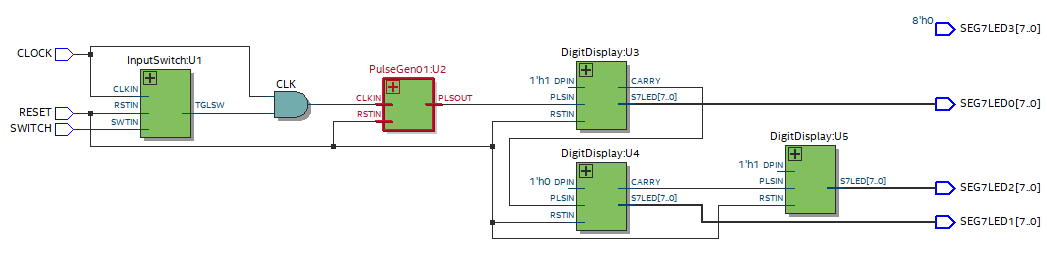
\includegraphics[width=\textwidth]{assets/RTL_All.png}
  \caption{StopWatchの全体像の回路}
\end{figure}

\begin{figure}[H]
  \centering
  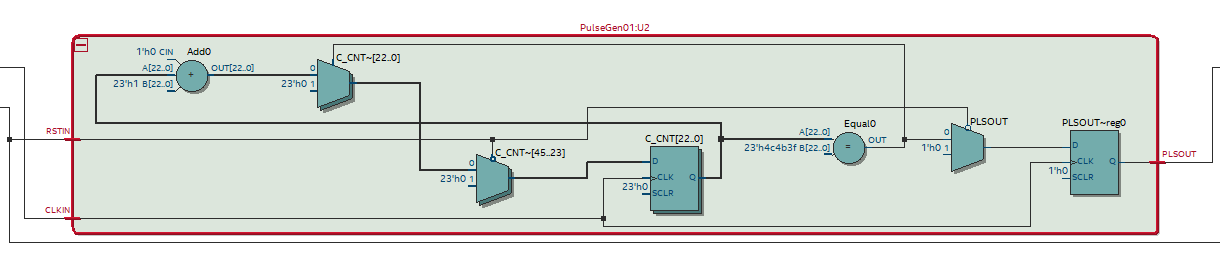
\includegraphics[width=\textwidth]{assets/RTL01.png}
  \caption{PulseGen01(同期式)の回路}
\end{figure}

\begin{figure}[H]
  \centering
  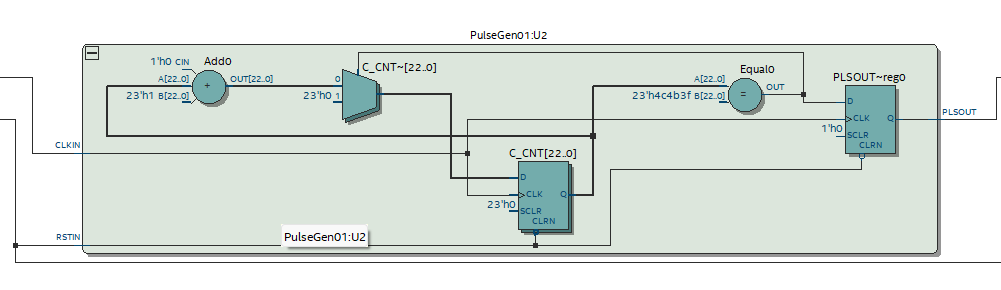
\includegraphics[width=\textwidth]{assets/RTL02.png}
  \caption{PulseGen01(非同期式)の回路}
\end{figure}

図3.5におけるPulseGen01:U2の内部構造が図3.6,3.7のようになっている。同期式の方が非同期式の回路より構成素子が多いことがわかる。
% 考察で書けそう
% これは、非同期式の方がリセット信号を直接的に扱うため、クロックイベントに依存せずに動作することができるからであると考えられる。

\subsubsection{StopWatchのSimulation結果}
図3.8, 3.9, 3.10にStopWatchのシミュレーション結果を示す。
各図のグラフには、上から順にCLOCK、INIT\_RESET、SWITCH、SEG7LED0、SEG7LED1、SEG7LED2が表示されている。
横軸(時間軸)を段階的に縮小することで、各SEG7LEDの動作タイミングを詳細に確認できるようにしている。

\begin{figure}[H]
  \centering
  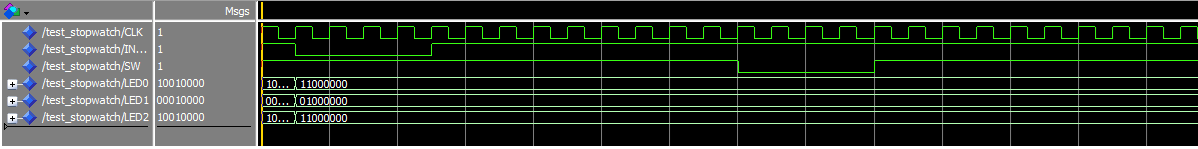
\includegraphics[width=\textwidth]{assets/simulation01.png}
  \caption{StopWatchのタイミングチャート(RESETとSWITCHのタイミング)}
\end{figure}

\begin{figure}[H]
  \centering
  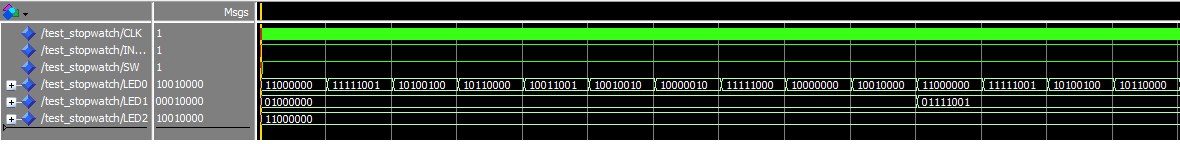
\includegraphics[width=\textwidth]{assets/simulation02.png}
  \caption{StopWatchのタイミングチャート(CLKとSEG7LED0,SEG7LED2のタイミング)}
\end{figure}

\begin{figure}[H]
  \centering
  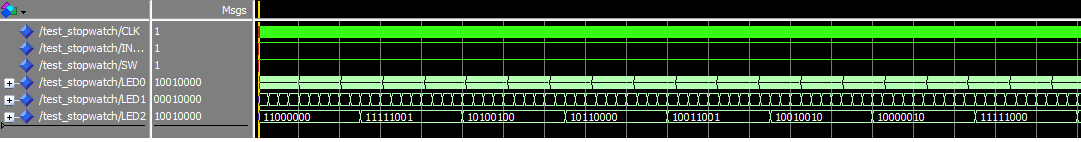
\includegraphics[width=\textwidth]{assets/simulation03.png}
  \caption{StopWatchのタイミングチャート(SEG7LED2とSEG7LED3のタイミング)}
\end{figure}

これらのタイミングチャートから、SEG7LED0は図3.11に示すSEG7LEDの数字表示に対応するように0から9までカウントを繰り返し、10回カウントされるごとにSEG7LED1に1つ桁上げされることが確認できる。同様に、SEG7LED1が10回カウントされるとSEG7LED2に1つ桁上げされる動作が見られる。

\begin{figure}[H]
  \centering
  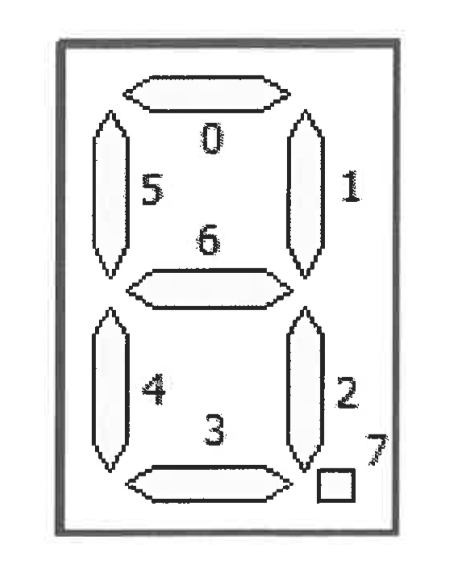
\includegraphics[width=0.2\textwidth]{assets/SEG7LED.png}
  \caption{SEG7LEDの表示}
\end{figure}

\section{考察}

\section{使用機材}
表5.1に示す。
\begin{table}[H]
  \centering
  \caption{使用機材一覧}
  \begin{tabular}{|c|c|c|c|}
    \hline
    名称 & 型式 & 製造元 & 管理番号 \\ \hline
    PC & & DELL &  \\ \hline
    FPGAボード & TERASIC-DE10-LITE-A P0466 & & \\ \hline
  \end{tabular}
\end{table}

\section{参考文献}
\begin{enumerate}
  \item FPGAとは, フィールドでプログラムできる論理回路 \\
    \url{https://jp.mathworks.com/discovery/fpga.html}\\
    閲覧日:2025年5月21日
  \item 新人エンジニアの赤面ブログ 『 RTL Viewer と Technology Map Viewer の使用用途を比べてみましょう』\\
    \url{https://www.macnica.co.jp/business/semiconductor/articles/intel/206/}\\
    閲覧日:2025年5月24日
\end{enumerate}

\end{document}